\chapter{The Riemann Hypothesis}
\label{ch:riemann}

\noindent\textbf{Key Ideas.}
\begin{itemize}
  \item The \emph{Riemann zeta function} $\zeta(s) = \sum_{n=1}^{\infty} n^{-s}$ encodes the distribution of prime numbers.
  \item The \emph{Euler product} $\zeta(s) = \prod_p (1 - p^{-s})^{-1}$ connects the zeta function to primes.
  \item The Riemann hypothesis asserts that all nontrivial zeros of $\zeta(s)$ lie on the \emph{critical line} $\Re(s) = \tfrac{1}{2}$.
  \item This would give the best possible error term in the prime number theorem.
\end{itemize}

\bigskip

\section{Introduction}

The Riemann hypothesis is, by almost universal consensus, the most important unsolved problem in pure mathematics. It concerns the distribution of prime numbers---the atoms of arithmetic---and encodes a profound symmetry in the behavior of the Riemann zeta function. Since its formulation by Bernhard Riemann in a landmark eight-page memoir in 1859, it has resisted all attempts at proof or disproof.

The problem appears on both of the most prestigious lists of open mathematical questions. David Hilbert included it as the eighth problem on his famous list of 23 problems, presented at the International Congress of Mathematicians in Paris in 1900. In 2000, the Clay Mathematics Institute designated it one of seven Millennium Prize Problems, each carrying a prize of one million dollars. Of those seven, only the Poincar\'{e} conjecture has been solved (by Grigori Perelman, who declined the prize). The Riemann hypothesis remains wide open.

Why does this problem captivate mathematicians so completely? The answer lies in the extraordinary web of connections that radiate from it. The Riemann hypothesis is equivalent to---or has deep implications for---an astonishing range of mathematical statements:

\begin{itemize}
  \item The distribution of prime numbers: how evenly are they spread among the integers?
  \item The growth rate of the error term in the prime number theorem.
  \item Bounds on prime gaps: how close can consecutive primes be?
  \item The behavior of many algorithms in computational number theory.
  \item The statistical properties of certain random matrices from nuclear physics.
  \item Deep questions in algebraic geometry over finite fields.
  \item The structure of the class numbers of quadratic fields.
  \item The distribution of eigenvalues of certain operators.
\end{itemize}

The hypothesis is remarkable not only for its depth but also for its simplicity. It can be stated in a single sentence, and its meaning can be roughly grasped by anyone who understands complex numbers. Yet proving it has turned out to be far beyond the reach of current mathematical techniques.

In this chapter, we will develop the theory of the Riemann zeta function from first principles, state the Riemann hypothesis precisely, explain its significance, survey the evidence for its truth, and discuss the progress that has been made over more than a century and a half of effort.

\section{Prime Numbers}
\label{sec:primes}

\subsection{Definition and the Fundamental Theorem}

A \textit{prime number} is a natural number $p > 1$ whose only positive divisors are $1$ and $p$. The first few primes are:
\[
2, \; 3, \; 5, \; 7, \; 11, \; 13, \; 17, \; 19, \; 23, \; 29, \; 31, \; 37, \; 41, \; 43, \; 47, \ldots
\]

The primes are the multiplicative building blocks of all positive integers, as guaranteed by the fundamental theorem of arithmetic:

\begin{theorem}[Fundamental theorem of arithmetic]
\label{thm:fta}
Every integer $n > 1$ can be written uniquely as a product of primes, up to the order of the factors:
\[
n = p_1^{a_1} p_2^{a_2} \cdots p_k^{a_k}
\]
where $p_1 < p_2 < \cdots < p_k$ are primes and $a_i \ge 1$.
\end{theorem}

\begin{proof}[Proof sketch]
Existence follows by strong induction: if $n$ is prime, we are done; if $n$ is composite, $n = ab$ with $1 < a, b < n$, and both $a$ and $b$ factor into primes by induction. Uniqueness relies on Euclid's lemma: if $p \mid ab$, then $p \mid a$ or $p \mid b$.
\end{proof}

\subsection{The Distribution of Primes}

While the fundamental theorem tells us that primes are the building blocks of the integers, it says nothing about \emph{how many} primes there are, or how they are distributed among the integers. The \textit{prime counting function} is defined by:
\[
\pi(x) = \#\{p \le x : p \text{ is prime}\}
\]

\begin{example}
$\pi(2) = 1$, \; $\pi(10) = 4$ (the primes $2, 3, 5, 7$), \; $\pi(100) = 25$, \; $\pi(1000) = 168$.
\end{example}

Even a cursory examination of the primes reveals puzzling irregularities. The gaps between consecutive primes vary wildly: $3 - 2 = 1$, $5 - 3 = 2$, $7 - 5 = 2$, $11 - 7 = 4$, $13 - 11 = 2$, and so on. There are arbitrarily long runs of composite numbers (for any $N$, the numbers $N!+2, N!+3, \ldots, N!+N$ are all composite), yet the twin prime conjecture asserts that there are infinitely many pairs of primes differing by $2$.

Despite this apparent randomness, the primes exhibit remarkable statistical regularity when viewed in the large. The study of this regularity is the central theme of analytic number theory.

\subsection{The Prime Number Theorem}

By the late eighteenth century, both Carl Friedrich Gauss and Adrien-Marie Legendre had independently conjectured that $\pi(x)$ is asymptotic to $x / \log x$:

\begin{conjecture}[Gauss--Legendre, c.\ 1793]
\label{conj:gauss}
\[
\pi(x) \sim \frac{x}{\log x} \quad \text{as } x \to \infty
\]
meaning $\displaystyle\lim_{x \to \infty} \frac{\pi(x)}{x / \log x} = 1$.
\end{conjecture}

Gauss arrived at this formula through extensive numerical experimentation. He computed tables of primes up to one million and noticed that $\pi(x)$ grew roughly like $x / \log x$. He also considered the logarithmic integral $\operatorname{Li}(x) = \int_2^x \frac{dt}{\log t}$, which provides a better approximation:
\[
\operatorname{Li}(x) = \frac{x}{\log x} + \frac{x}{(\log x)^2} + \frac{2x}{(\log x)^3} + \cdots
\]

Legendre published a slightly different version in 1798, claiming $\pi(x) \approx \frac{x}{\log x - 1.08366}$, which is a less elegant approximation but remarkably accurate for moderate values of $x$.

The conjecture stood for over a century before it was proved in 1896, independently and almost simultaneously by Jacques Hadamard and Charles Jean de la Vall\'{e}e Poussin:

\begin{theorem}[Prime number theorem]
\label{thm:pnt}
\[
\lim_{x \to \infty} \frac{\pi(x)}{x / \log x} = 1
\]
\end{theorem}

Both proofs used complex analysis---specifically, properties of the Riemann zeta function and the fact that $\zeta(s) \neq 0$ on the line $\mathbb{R}e(s) = 1$. This was the first indication of the profound connection between the zeros of $\zeta(s)$ and the distribution of primes.

A weaker form was proved earlier by Chebyshev (1852), who showed that there exist constants $0 < c < C$ such that:
\[
c \cdot \frac{x}{\log x} \le \pi(x) \le C \cdot \frac{x}{\log x}
\]

\begin{exercise}
\label{ex:pi100}
Compute $\pi(x)$ for $x = 10, 20, 50, 100$ by hand. Compare with $x / \log x$ and $\operatorname{Li}(x)$.
\end{exercise}

\begin{exercise}
\label{ex:chebyshev}
Prove Chebyshev's upper bound $\pi(x) \le \frac{3}{2} \cdot \frac{x}{\log x}$ for $x \ge 4$ by estimating $\binom{2n}{n} = \frac{(2n)!}{(n!)^2}$ and using the fact that this binomial coefficient is divisible by the product of all primes $n < p \le 2n$.
\end{exercise}

\begin{exercise}
\label{ex:primegaps}
Prove that for any positive integer $N$, there exist $N$ consecutive composite numbers. (Hint: consider $N! + 2, N! + 3, \ldots, N! + N$.)
\end{exercise}

\section{The Riemann Zeta Function}
\label{sec:zeta}

\subsection{Definition and Basic Properties}

The Riemann zeta function is defined by a Dirichlet series:

\begin{definition}
For a complex variable $s = \sigma + it$ with $\mathbb{R}e(s) = \sigma > 1$, the \textit{Riemann zeta function} is:
\[
\zeta(s) = \sum_{n=1}^{\infty} \frac{1}{n^s}
\]
\end{definition}

\begin{proposition}
\label{prop:zeta_conv}
The series defining $\zeta(s)$ converges absolutely for $\mathbb{R}e(s) > 1$ and uniformly on compact subsets of this half-plane.
\end{proposition}

\begin{proof}
We have $\left|\frac{1}{n^s}\right| = \frac{1}{n^{\sigma}}$. The $p$-series $\sum n^{-\sigma}$ converges for $\sigma > 1$ by the integral test. Uniform convergence on compact subsets follows from the Weierstrass M-test, since for any $K \subset \{s : \mathbb{R}e(s) > 1\}$ compact, there exists $\sigma_0 > 1$ with $\mathbb{R}e(s) \ge \sigma_0$ for all $s \in K$.
\end{proof}

Since the terms are holomorphic in $s$ and the series converges uniformly on compact subsets, $\zeta(s)$ is a \textit{holomorphic function} on the half-plane $\mathbb{R}e(s) > 1$.

\begin{example}
$\zeta(2) = \sum_{n=1}^{\infty} \frac{1}{n^2} = 1 + \frac{1}{4} + \frac{1}{9} + \frac{1}{16} + \cdots = \frac{\pi^2}{6}$

This famous identity was first proved by Euler in 1734. It tells us that the sum of the reciprocals of all perfect squares equals exactly $\pi^2 / 6 \approx 1.6449\ldots$
\end{example}

\begin{example}
$\zeta(3) = \sum_{n=1}^{\infty} \frac{1}{n^3} \approx 1.2021\ldots$

This number is called \textit{Ap\'{e}ry's constant}. Ap\'{e}ry proved in 1978 that $\zeta(3)$ is irrational, but whether $\zeta(3) / \pi^3$ is irrational (or even whether $\zeta(3)$ is transcendental) remains unknown.
\end{example}

\begin{example}
$\zeta(4) = \frac{\pi^4}{90}$, \quad $\zeta(6) = \frac{\pi^6}{945}$, \quad $\zeta(2k) = \frac{(-1)^{k+1} B_{2k} (2\pi)^{2k}}{2(2k)!}$

where $B_{2k}$ are Bernoulli numbers. In general, $\zeta(2k)$ is a rational multiple of $\pi^{2k}$.
\end{example}

\subsection{The Euler Product}

The deepest property of the zeta function---and the reason it is relevant to prime numbers---is the Euler product formula. This identity expresses $\zeta(s)$ as a product over all primes:

\begin{theorem}[Euler product]
\label{thm:euler}
For $\mathbb{R}e(s) > 1$:
\[
\zeta(s) = \prod_{p \text{ prime}} \left(1 - p^{-s}\right)^{-1}
\]
\end{theorem}

\begin{proof}
For a fixed $\mathbb{R}e(s) > 1$, consider the finite product over all primes $p \le N$:
\[
P_N(s) = \prod_{p \le N} \left(1 - p^{-s}\right)^{-1}
\]
Each factor is a geometric series:
\[
\left(1 - p^{-s}\right)^{-1} = \sum_{k=0}^{\infty} p^{-ks} = 1 + p^{-s} + p^{-2s} + p^{-3s} + \cdots
\]
Multiplying these geometric series together for all primes $p \le N$:
\[
P_N(s) = \prod_{p \le N} \sum_{k=0}^{\infty} p^{-ks}
\]
When we expand this product, each term in the expansion has the form $\prod_{p \le N} p^{-k_p s} = n^{-s}$ where $n = \prod_{p \le N} p^{k_p}$. By the fundamental theorem of arithmetic, each positive integer $n$ whose prime factors are all $\le N$ appears exactly once. Therefore:
\[
P_N(s) = \sum_{\substack{n=1 \\ \text{all prime factors of } n \le N}}^{\infty} n^{-s}
\]
This is a partial sum of the Dirichlet series for $\zeta(s)$, plus possibly some additional terms. More precisely:
\[
P_N(s) = \zeta(s) - \sum_{\substack{n=1 \\ n \text{ has a prime factor} > N}}^{\infty} n^{-s}
\]
For the error term, we estimate:
\[
\left|\sum_{\substack{n \text{ has a prime factor} > N}} n^{-s}\right| \le \sum_{n > N} n^{-\sigma} \le \int_N^{\infty} x^{-\sigma} \, dx = \frac{N^{1-\sigma}}{\sigma - 1} \to 0 \quad \text{as } N \to \infty
\]
since $\sigma > 1$. Therefore $\lim_{N \to \infty} P_N(s) = \zeta(s)$, which establishes the identity.
\end{proof}

\begin{figure}[htbp]
\centering
\begin{tikzpicture}[
  node distance=1.8cm,
  every node/.style={align=center},
  box/.style={draw, rounded corners, minimum width=2.2cm, minimum height=0.8cm, font=\small},
  primebox/.style={draw, rectangle, minimum width=2.8cm, minimum height=0.7cm, font=\small}
]
  % Central zeta node
  \node[box, fill=blue!10, minimum width=2.5cm] (zeta) {$\displaystyle\zeta(s)$};
  % Arrow down
  \node[below=1.5cm of zeta] (eq) {\large $=$};
  % Prime factors
  \node[primebox, below left=1.2cm and 3.0cm of eq] (p2) {$\left(1 - 2^{-s}\right)^{-1}$};
  \node[primebox, below left=1.2cm and 0.3cm of eq] (p3) {$\left(1 - 3^{-s}\right)^{-1}$};
  \node[primebox, below right=1.2cm and 0.3cm of eq] (p5) {$\left(1 - 5^{-s}\right)^{-1}$};
  \node[primebox, below right=1.2cm and 3.0cm of eq] (p7) {$\left(1 - 7^{-s}\right)^{-1}$};
  % Dots
  \node[below=2.5cm of eq] (dots) {\large $\cdots$};
  % Multiplication signs
  \node[below=0.6cm of zeta] (times1) {\large $\displaystyle\prod_{p\text{ prime}}$};
  % Draw arrows from zeta
  \draw[->,thick] (zeta) -- (p2) node[midway,left,font=\small] {\large$\times$};
  \draw[->,thick] (zeta) -- (p3) node[midway,left,font=\small, xshift=-0.1cm] {\large$\times$};
  \draw[->,thick] (zeta) -- (p5) node[midway,right,font=\small, xshift=0.1cm] {\large$\times$};
  \draw[->,thick] (zeta) -- (p7) node[midway,right,font=\small] {\large$\times$};
  \draw[->,thick] (zeta) -- (dots);
  % Labels
  \node[below=0.1cm of p2, font=\scriptsize] {prime $p=2$};
  \node[below=0.1cm of p3, font=\scriptsize] {prime $p=3$};
  \node[below=0.1cm of p5, font=\scriptsize] {prime $p=5$};
  \node[below=0.1cm of p7, font=\scriptsize] {prime $p=7$};
\end{tikzpicture}
\caption{The Euler product decomposes the zeta function into a product over all primes. Each prime $p$ contributes a local factor $(1 - p^{-s})^{-1}$, encoding all information about divisibility by $p$.}
\label{fig:euler_product}
\end{figure}

\begin{checkyou}
\begin{enumerate}
  \item Can you explain in your own words why the Euler product encodes all information about primes?
  \item If you set $s = 2$ in the Euler product and take the first 100 primes, how close is the result to $\pi^2/6$?
\end{enumerate}
\end{checkyou}

\begin{example}[Numerical verification of the Euler product at $s=2$]
\label{ex:eulerprod_numerical}
We verify the Euler product formula for $\zeta(2) = \pi^2/6$ by computing partial products over the first few primes.

\textbf{The identity to check.} Setting $s = 2$ in the Euler product:
\[
\zeta(2) = \prod_{p \text{ prime}} \left(1 - \frac{1}{p^2}\right)^{-1} = \frac{\pi^2}{6} \approx 1.644934\ldots
\]

\textbf{Step-by-step computation.} We build the product one prime at a time. For each prime $p$, the factor is $(1 - p^{-2})^{-1} = p^2/(p^2 - 1)$.

\medskip
\noindent\textbf{Prime $p = 2$:}\quad $\displaystyle\left(1 - \frac{1}{4}\right)^{-1} = \frac{4}{3} = 1.333333\ldots$

\noindent\textbf{Primes $2, 3$:}\quad $\displaystyle\frac{4}{3} \cdot \left(1 - \frac{1}{9}\right)^{-1} = \frac{4}{3} \cdot \frac{9}{8} = \frac{36}{24} = \frac{3}{2} = 1.500000$

\noindent\textbf{Primes $2, 3, 5$:}\quad $\displaystyle\frac{3}{2} \cdot \left(1 - \frac{1}{25}\right)^{-1} = \frac{3}{2} \cdot \frac{25}{24} = \frac{75}{48} = \frac{25}{16} = 1.562500$

\noindent\textbf{Primes $2, 3, 5, 7$:}\quad $\displaystyle\frac{25}{16} \cdot \left(1 - \frac{1}{49}\right)^{-1} = \frac{25}{16} \cdot \frac{49}{48} = \frac{1225}{768} \approx 1.595052$

\noindent\textbf{Primes $2, 3, 5, 7, 11$:}\quad $\displaystyle\frac{1225}{768} \cdot \frac{121}{120} = \frac{148225}{92160} \approx 1.608353$

\noindent\textbf{Primes up to $29$:}\quad $\approx 1.614775$

\noindent\textbf{Primes up to $97$:}\quad $\approx 1.632849$

\noindent\textbf{Primes up to $997$:}\quad $\approx 1.643844$

\noindent\textbf{Primes up to $9973$:}\quad $\approx 1.644799$

\medskip
\noindent Comparing with the target:
\[
\frac{\pi^2}{6} \approx 1.644934
\]
After including all primes up to $9973$ (the first $1229$ primes), the partial product agrees with $\pi^2/6$ to better than $0.07\%$. The convergence is steady and monotone (each factor is $> 1$, so the partial products increase toward $\pi^2/6$).

\textbf{Why it works.} Each factor $(1 - p^{-2})^{-1} > 1$ accounts for the contributions of all powers $p, p^2, p^3, \ldots$ of that prime to the sum $\sum n^{-2}$. The product converges because $\sum_p p^{-2}$ converges (a sum over primes is always dominated by the corresponding sum over all integers).
\end{example}

\begin{remark}
The Euler product is often called the ``golden key'' of number theory. It expresses the fact that the zeta function encodes all arithmetic information about the primes. Any property of $\zeta(s)$ translates into a property of the primes, and vice versa.
\end{remark}

\begin{corollary}
\label{cor:infprime}
The Euler product gives a new proof that there are infinitely many primes: if there were only finitely many, the product would be a finite product of convergent factors, giving an analytic function everywhere. But $\zeta(s)$ has a pole at $s = 1$ (as we will show), contradicting this.
\end{corollary}

\begin{exercise}
\label{ex:eulerprod}
Verify the Euler product numerically for $s = 2$: compute $\prod_{p \le 1000} (1 - p^{-2})^{-1}$ and compare with $\pi^2 / 6$.
\end{exercise}

\begin{exercise}
\label{ex:eulerprod3}
Use the Euler product to show that $\sum_{p} p^{-2}$ converges, where the sum is over all primes. Show that $\sum_p p^{-1}$ diverges. (Hint: take logarithms of the Euler product at $s = 1 + \epsilon$ and let $\epsilon \to 0^+$.)
\end{exercise}

\subsection{The Gamma Function}

To understand the analytic continuation of $\zeta(s)$, we need the Gamma function, which generalizes the factorial to complex arguments.

\begin{definition}
For $\mathbb{R}e(z) > 0$, the \textit{Gamma function} is defined by:
\[
\Gamma(z) = \int_0^{\infty} t^{z-1} e^{-t} \, dt
\]
\end{definition}

The Gamma function satisfies the functional equation $z \Gamma(z) = \Gamma(z+1)$, which implies $\Gamma(n) = (n-1)!$ for positive integers $n$. It extends to a meromorphic function on all of $\mathbb{C}$ with simple poles at $z = 0, -1, -2, \ldots$ and no zeros.

Key properties we will need:
\begin{itemize}
  \item $\Gamma(1/2) = \sqrt{\pi}$
  \item The reflection formula: $\Gamma(z)\Gamma(1-z) = \pi / \sin(\pi z)$
  \item The duplication formula: $\Gamma(z)\Gamma(z + 1/2) = 2^{1-2z} \sqrt{\pi} \, \Gamma(2z)$
\end{itemize}

\subsection{The Functional Equation and Analytic Continuation}

Riemann's great insight was to extend $\zeta(s)$ to the entire complex plane and to discover a functional equation relating $\zeta(s)$ to $\zeta(1-s)$. There are several ways to derive this; the most classical uses the theta function and the Poisson summation formula.

\begin{definition}
The \textit{completed zeta function} (or \textit{xi function}) is:
\[
\xi(s) = \pi^{-s/2} \Gamma\left(\frac{s}{2}\right) \zeta(s)
\]
\end{definition}

\begin{theorem}[Functional equation of $\zeta(s)$]
\label{thm:func}
The completed zeta function satisfies:
\[
\xi(s) = \xi(1-s)
\]
Equivalently, for all $s \in \mathbb{C}$ (except $s = 0$ and $s = 1$):
\[
\zeta(s) = 2^s \pi^{s-1} \sin\left(\frac{\pi s}{2}\right) \Gamma(1-s) \, \zeta(1-s)
\]
\end{theorem}

\begin{checkyou}
\begin{enumerate}
  \item Why does $\xi(s) = \xi(1-s)$ imply symmetry about $\Re(s) = 1/2$?
  \item If you know the values of $\zeta(s)$ for $\Re(s) > 1/2$, can you determine $\zeta(s)$ for $\Re(s) < 1/2$? Why or why not?
\end{enumerate}
\end{checkyou}

\begin{proof}[Proof outline]
The derivation proceeds in three steps.

\textbf{Step 1.} Start with the integral representation for $\mathbb{R}e(s) > 1$:
\[
\Gamma\left(\frac{s}{2}\right) \zeta(s) = \int_0^{\infty} \left(\sum_{n=1}^{\infty} e^{-\pi n^2 t}\right) t^{s/2} \frac{dt}{t}
\]

\textbf{Step 2.} Apply the Poisson summation formula to the theta function $\theta(t) = \sum_{n=-\infty}^{\infty} e^{-\pi n^2 t}$ to obtain:
\[
\theta(t) = t^{-1/2} \, \theta(1/t)
\]
This is the modularity of the theta function. Decompose $\theta(t) = 1 + 2\sum_{n=1}^{\infty} e^{-\pi n^2 t}$ and split the integral at $t = 1$.

\textbf{Step 3.} After substitution $t \mapsto 1/t$ in the integral from $1$ to $\infty$, one obtains:
\[
\pi^{-s/2} \Gamma\left(\frac{s}{2}\right) \zeta(s) = \frac{1}{s(s-1)} + \int_1^{\infty} \left(t^{s/2} + t^{(1-s)/2}\right) \psi(t) \, dt
\]
where $\psi(t) = \sum_{n=1}^{\infty} e^{-\pi n^2 t}$. The right-hand side is manifestly invariant under $s \mapsto 1-s$.
\end{proof}

\begin{remark}
The functional equation reveals that the zeta function has a perfect symmetry about the line $\mathbb{R}e(s) = 1/2$. If we know $\zeta(s)$ in the half-plane $\mathbb{R}e(s) > 1/2$, we know it everywhere.
\end{remark}

\begin{theorem}[Analytic continuation]
\label{thm:analytic}
The Riemann zeta function extends to a meromorphic function on all of $\mathbb{C}$ with a single simple pole at $s = 1$ with residue $1$.
\end{theorem}

\begin{proof}[Proof sketch]
For $\mathbb{R}e(s) > 1$, the series $\sum n^{-s}$ converges. For $\mathbb{R}e(s) \le 1$, the functional equation (Theorem~\ref{thm:func}) expresses $\zeta(s)$ in terms of $\zeta(1-s)$, where $1-s$ has $\mathbb{R}e(1-s) > 1$ when $\mathbb{R}e(s) < 0$. The case $0 \le \mathbb{R}e(s) \le 1$ (the critical strip) requires a more careful argument, typically using a contour integral representation:
\[
\zeta(s) = \frac{\Gamma(1-s)}{2\pi i} \int_C \frac{(-z)^{s-1}}{e^z - 1} \, dz
\]
where $C$ is a contour encircling the positive real axis. This representation converges for all $s \neq 1$ and gives a meromorphic continuation. The simple pole at $s = 1$ comes from the residue at $z = 0$.
\end{proof}

\begin{exercise}
\label{ex:zeta_neg_even}
Use the functional equation to show that $\zeta(-2n) = 0$ for all positive integers $n$. These are called the \textit{trivial zeros} of $\zeta(s)$.
\end{exercise}

\begin{exercise}
\label{ex:zeta_neg1}
Use the functional equation and the reflection formula $\Gamma(z)\Gamma(1-z) = \pi / \sin(\pi z)$ to prove that $\zeta(-1) = -\frac{1}{12}$. Explain why this does \emph{not} mean that $1 + 2 + 3 + 4 + \cdots = -\frac{1}{12}$ in the usual sense.
\end{exercise}

\section{Zeros of the Zeta Function}
\label{sec:zeros}

The zeros of $\zeta(s)$ are central to the Riemann hypothesis. The functional equation and the properties of the Gamma and sine functions tell us exactly where all zeros must lie.

\subsection{Trivial Zeros}

The functional equation $\zeta(s) = 2^s \pi^{s-1} \sin(\pi s / 2) \, \Gamma(1-s) \, \zeta(1-s)$ contains the factor $\sin(\pi s / 2)$, which vanishes at $s = -2, -4, -6, \ldots$ At these points, $\Gamma(1-s)$ has poles (at $s = 0, -2, -4, \ldots$), but the poles of $\Gamma(1-s)$ at the negative even integers are canceled by the zeros of $\sin(\pi s / 2)$, and the resulting product yields zeros of $\zeta(s)$:

\begin{theorem}
The \textit{trivial zeros} of $\zeta(s)$ are exactly the negative even integers $s = -2, -4, -6, \ldots$ Each is a simple zero.
\end{theorem}

At these points, $\zeta(-2n) = 0$ for $n = 1, 2, 3, \ldots$

\subsection{The Critical Strip and the Critical Line}

All remaining zeros of $\zeta(s)$ lie in the \textit{critical strip} $0 < \mathbb{R}e(s) < 1$. This follows from the fact that $\zeta(s) \neq 0$ for $\mathbb{R}e(s) > 1$ (which can be proved from the Euler product) and from $\mathbb{R}e(s) < 0$ (where the only zeros are the trivial ones, via the functional equation). The zeros in the critical strip are called \textit{non-trivial zeros}.

\begin{checkyou}
\begin{enumerate}
  \item Why can there be no zeros outside the critical strip other than the trivial ones?
  \item What happens to $\zeta(s)$ on the line $\Re(s) = 1$? Why is this important for the prime number theorem?
\end{enumerate}
\end{checkyou}

By the functional equation $\xi(s) = \xi(1-s)$, if $\rho$ is a non-trivial zero, then $1 - \rho$ is also a non-trivial zero. The zeros are symmetric about the line $\mathbb{R}e(s) = 1/2$.

\begin{definition}
The \textit{critical line} is the line $\mathbb{R}e(s) = \frac{1}{2}$ in the complex plane.
\end{definition}

\begin{figure}[htbp]
\centering
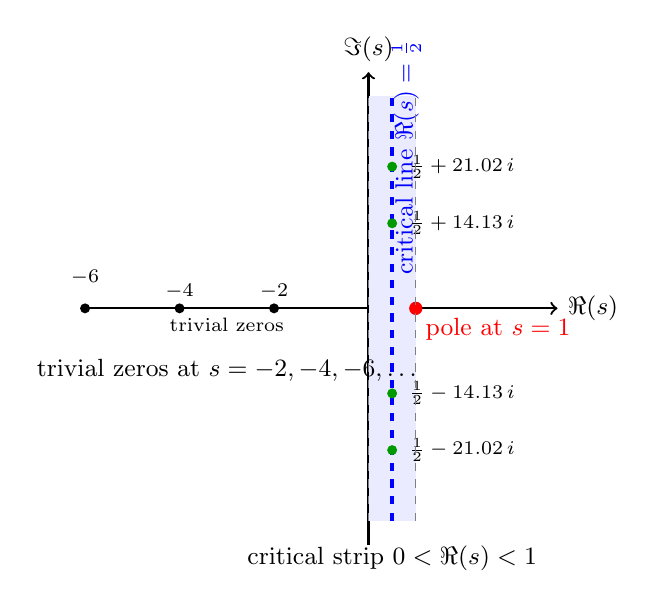
\begin{tikzpicture}[scale=0.6]
  % Axes
  \draw[->,thick] (-6,0) -- (4,0) node[right] {\small $\Re(s)$};
  \draw[->,thick] (0,-5) -- (0,5) node[above] {\small $\Im(s)$};
  % Critical strip shaded
  \fill[blue!8] (0,-4.5) rectangle (1,4.5);
  % Critical line
  \draw[blue,very thick,dashed] (0.5,-4.5) -- (0.5,4.5);
  \node[blue,font=\small,rotate=90] at (0.8,3.2) {critical line $\Re(s)=\frac{1}{2}$};
  % Pole at s=1
  \fill[red] (1,0) circle (4pt);
  \node[below right,red] at (1,0) {\small pole at $s=1$};
  % Trivial zeros
  \fill[black] (-2,0) circle (3pt);
  \node[above,font=\scriptsize] at (-2,0) {$-2$};
  \fill[black] (-4,0) circle (3pt);
  \node[above,font=\scriptsize] at (-4,0) {$-4$};
  \fill[black] (-6,0) circle (3pt);
  \node[above,font=\scriptsize] at (-6,0.3) {$-6$};
  \node[below,font=\scriptsize] at (-3,0) {trivial zeros};
  % Non-trivial zeros on critical line
  \fill[green!60!black] (0.5,1.8) circle (3pt);
  \fill[green!60!black] (0.5,3.0) circle (3pt);
  \fill[green!60!black] (0.5,-1.8) circle (3pt);
  \fill[green!60!black] (0.5,-3.0) circle (3pt);
  \node[right,font=\scriptsize] at (0.65,1.8) {$\frac{1}{2}+14.13\,i$};
  \node[right,font=\scriptsize] at (0.65,3.0) {$\frac{1}{2}+21.02\,i$};
  \node[right,font=\scriptsize] at (0.65,-1.8) {$\frac{1}{2}-14.13\,i$};
  \node[right,font=\scriptsize] at (0.65,-3.0) {$\frac{1}{2}-21.02\,i$};
  % Labels
  \node[font=\small] at (0.5,-5.3) {critical strip $0 < \Re(s) < 1$};
  \node[font=\small] at (-3,-1.3) {trivial zeros at $s=-2,-4,-6,\ldots$};
  % Re(s)=1 line
  \draw[gray,thin,dashed] (1,-4.5) -- (1,4.5);
  % Re(s)=0 line (imaginary axis)
  \draw[gray,thin,dashed] (0,-4.5) -- (0,4.5);
\end{tikzpicture}
\caption{The critical strip and critical line in the complex plane. The Riemann hypothesis asserts that all non-trivial zeros of $\zeta(s)$ lie on the dashed critical line $\Re(s) = \frac{1}{2}$. The trivial zeros lie at the negative even integers.}
\label{fig:critical_strip}
\end{figure}

The Riemann hypothesis asserts:

\begin{theorem}[Riemann hypothesis]
\label{thm:rh}
All non-trivial zeros of the Riemann zeta function have real part equal to $\frac{1}{2}$. That is, if $\zeta(\rho) = 0$ and $\rho$ is non-trivial, then $\mathbb{R}e(\rho) = \frac{1}{2}$.
\end{theorem}

In other words, every non-trivial zero lies on the critical line. Equivalently:
\[
\text{If } \zeta(\rho) = 0 \text{ and } 0 < \mathbb{R}e(\rho) < 1, \text{ then } \rho = \frac{1}{2} + it \text{ for some } t \in \mathbb{R}.
\]

\begin{example}[Computing $\zeta(-1) = -\tfrac{1}{12}$ via the functional equation]
\label{ex:zeta_neg1_worked}
We use the functional equation to evaluate $\zeta$ at the negative odd integer $s = -1$, arriving at the famous identity $1 + 2 + 3 + \cdots \;\overset{?}{=}\; -\tfrac{1}{12}$.

\textbf{The functional equation.} Recall (Theorem~\ref{thm:func}):
\[
\zeta(s) = 2^s \, \pi^{s-1} \, \sin\!\left(\frac{\pi s}{2}\right) \, \Gamma(1 - s) \, \zeta(1 - s)
\]

\textbf{Step 1: Substitute $s = -1$.}
\[
\zeta(-1) = 2^{-1} \cdot \pi^{-2} \cdot \sin\!\left(\frac{-\pi}{2}\right) \cdot \Gamma(2) \cdot \zeta(2)
\]

\textbf{Step 2: Evaluate each factor.}
\begin{itemize}
  \item $2^{-1} = \dfrac{1}{2}$
  \item $\pi^{-2} = \dfrac{1}{\pi^2}$
  \item $\sin\!\left(\dfrac{-\pi}{2}\right) = -1$
  \item $\Gamma(2) = 1! = 1$ \quad (using $\Gamma(n) = (n-1)!$ for positive integers)
  \item $\zeta(2) = \dfrac{\pi^2}{6}$ \quad (Euler's Basel problem result)
\end{itemize}

\textbf{Step 3: Multiply.}
\[
\zeta(-1) = \frac{1}{2} \cdot \frac{1}{\pi^2} \cdot (-1) \cdot 1 \cdot \frac{\pi^2}{6} = -\frac{1}{2} \cdot \frac{1}{6} = -\frac{1}{12}
\]

\textbf{Remark on the ``sum'' $1 + 2 + 3 + \cdots$.}
The Dirichlet series $\zeta(s) = \sum_{n=1}^{\infty} n^{-s}$ converges only for $\Re(s) > 1$. The value $\zeta(-1) = -1/12$ is obtained by \emph{analytic continuation}---it is \emph{not} the sum of the divergent series $1 + 2 + 3 + \cdots$ in the usual sense of partial sums. However, it is the unique value assigned by the analytic continuation, and it appears in physical calculations (such as the Casimir effect and bosonic string theory) where a regularization of the divergent sum is needed.
\end{example}

\begin{remark}
If a zero $\rho$ with $\mathbb{R}e(\rho) \neq 1/2$ existed, then by the functional equation, $1 - \overline{\rho}$ would also be a zero (since $\zeta(\overline{s}) = \overline{\zeta(s)}$ for real $s$, and this extends to all $s$). The point $1 - \overline{\rho}$ has real part $1 - \mathbb{R}e(\rho) \neq 1/2$ as well, so zeros off the critical line would come in quadruples (or pairs, if they lie on the real axis, which they do not in the critical strip).
\end{remark}

\subsection{The Riemann--von Mangoldt Formula}

The distribution of zeros is precisely counted by the Riemann--von Mangoldt formula. Let $N(T)$ denote the number of non-trivial zeros $\rho$ with $0 < \Im(\rho) \le T$:

\begin{theorem}[Riemann--von Mangoldt formula]
\label{thm:rvm}
\[
N(T) = \frac{T}{2\pi} \log\frac{T}{2\pi} - \frac{T}{2\pi} + O(\log T)
\]
\end{theorem}

This formula counts zeros up to height $T$ in the critical strip. It tells us that:
\begin{itemize}
  \item The number of zeros grows roughly like $\frac{T}{2\pi} \log T$.
  \item The average spacing between consecutive zeros near height $T$ is approximately $\frac{2\pi}{\log T}$.
  \item The zeros become denser as we move up the critical strip.
\end{itemize}

The Riemann--von Mangoldt formula is proved by applying the argument principle to $\zeta(s)$ on a rectangular contour bounding the critical strip up to height $T$. The key step is computing the change in argument of $\zeta(s)$ along the contour, which requires careful asymptotic analysis of $\zeta(s)$ on the boundaries.

\subsection{Visual Description of the Zeros}

The first few non-trivial zeros of $\zeta(s)$ are:
\[
\rho_1 = \frac{1}{2} + 14.134725\ldots i, \quad \rho_2 = \frac{1}{2} + 21.022040\ldots i, \quad \rho_3 = \frac{1}{2} + 25.010858\ldots i
\]
All computed zeros lie on the critical line. The imaginary parts of the first several zeros (up to $\Im(\rho) \approx 100$) are:
\[
14.13,\; 21.02,\; 25.01,\; 30.42,\; 32.94,\; 37.59,\; 40.92,\; 43.33,\; 48.01,\; 49.77, \ldots
\]

The gaps between consecutive zeros are not uniform but exhibit a statistical regularity that has been compared to the eigenvalue spacings of random matrices (a connection we discuss in Section~\ref{sec:montgomery}).

If one plots the function $|\zeta(1/2 + it)|$ for $t \in [0, T]$, the graph oscillates wildly, crossing zero frequently. The zeros are the points where the graph touches the horizontal axis. The distribution of these crossings, while not periodic, has a strikingly regular statistical character.

\begin{exercise}
\label{ex:nontropos}
Show that $\zeta(s)$ has no zeros with $\mathbb{R}e(s) > 1$. (Hint: use the Euler product and the fact that $\log \zeta(s) = \sum_p \sum_{k=1}^{\infty} \frac{1}{k p^{ks}}$ for $\mathbb{R}e(s) > 1$.)
\end{exercise}

\begin{exercise}
\label{ex:symmetry}
Prove that if $\rho$ is a non-trivial zero of $\zeta(s)$, then so is $1 - \overline{\rho}$. Deduce that non-trivial zeros off the critical line come in quadruples $\rho, \overline{\rho}, 1-\rho, 1-\overline{\rho}$.
\end{exercise}

\section{The Prime Number Theorem and the Error Term}
\label{sec:pnt_error}

\subsection{From Zeta to Primes: The Proof Sketch of PNT}

The prime number theorem (Theorem~\ref{thm:pnt}) states that $\pi(x) \sim x / \log x$. The modern proof, following Hadamard and de la Vall\'{e}e Poussin, connects $\pi(x)$ to the zeros of $\zeta(s)$ via the von Mangoldt function:

\begin{definition}
The \textit{von Mangoldt function} is:
\[
\Lambda(n) = \begin{cases} \log p & \text{if } n = p^k \text{ for some prime } p \text{ and } k \ge 1, \\ 0 & \text{otherwise.} \end{cases}
\]
\end{definition}

The related summatory function is:
\[
\psi(x) = \sum_{n \le x} \Lambda(n) = \sum_{p^k \le x} \log p
\]

The key relationship is:
\[
\pi(x) = \sum_{p \le x} 1 = \frac{\psi(x)}{\log x} + \int_2^x \frac{\psi(t)}{t(\log t)^2} \, dt + O(1)
\]
so understanding $\psi(x)$ gives information about $\pi(x)$.

The proof of the prime number theorem requires showing that $\zeta(s) \neq 0$ on the line $\mathbb{R}e(s) = 1$:

\begin{theorem}[Hadamard--de la Vall\'{e}e Poussin]
\label{thm:nozeroline1}
$\zeta(1 + it) \neq 0$ for all $t \in \mathbb{R}$.
\end{theorem}

\begin{proof}[Proof sketch]
Suppose $\zeta(1 + it_0) = 0$ for some $t_0 \neq 0$. Then $\zeta(1 - it_0) = 0$ as well (by the functional equation and $\overline{\zeta(s)} = \zeta(\overline{s})$). For $s$ near $1$, the Euler product would give:
\[
\zeta(s) \approx (s - 1)^2 \cdot (\text{nonvanishing factor})
\]
since $\zeta(s)$ has a simple pole at $s = 1$. But $\zeta(s)^3 |\zeta(s + it_0)|^2$ would then behave like $(s-1)^{-1}$ near $s = 1$, which is impossible because $\zeta(s)^3 |\zeta(s+it_0)|^2$ can be expressed as a Dirichlet series with non-negative coefficients, and such a series cannot have a pole of order other than what comes from the simple pole of $\zeta(s)$.
\end{proof}

From the non-vanishing on $\mathbb{R}e(s) = 1$, the explicit formula (discussed in Section~\ref{sec:explicit}) gives:
\[
\psi(x) = x + O(x \cdot e^{-c\sqrt{\log x}})
\]
for some constant $c > 0$. This implies $\pi(x) \sim \operatorname{Li}(x)$.

\subsection{The Error Term and the Riemann Hypothesis}

The quality of the approximation $\pi(x) \approx \operatorname{Li}(x)$ depends directly on where the zeros of $\zeta(s)$ lie. In general:

\[
\pi(x) = \operatorname{Li}(x) - \sum_{\rho} \operatorname{Li}(x^{\rho}) + \text{(smaller terms)}
\]

where the sum is over all non-trivial zeros $\rho$ of $\zeta(s)$. If the Riemann hypothesis is true, every zero satisfies $\mathbb{R}e(\rho) = 1/2$, and each term $\operatorname{Li}(x^{\rho})$ contributes at most $O(\sqrt{x})$ to the error. This gives:

\begin{theorem}
Assuming the Riemann hypothesis:
\[
\pi(x) = \operatorname{Li}(x) + O(\sqrt{x} \, \log x)
\]
\end{theorem}

Without the Riemann hypothesis, the best known unconditional bound is:

\begin{theorem}[Vinogradov--Korobov, 1958]
\[
\pi(x) = \operatorname{Li}(x) + O\left(x \exp\left(-c (\log x)^{3/5} (\log\log x)^{-1/5}\right)\right)
\]
for some absolute constant $c > 0$.
\end{theorem}

This is a significant improvement over $O(x / \log x)$ (which follows from Chebyshev-type bounds) but far weaker than what the Riemann hypothesis would give. The gap between the known error term and the conjectured error term is a measure of how much information about the zeros we are missing.

\subsection{Li$(x)$ vs.\ $\pi(x)$}

The logarithmic integral $\operatorname{Li}(x) = \int_2^x \frac{dt}{\log t}$ is a better approximation to $\pi(x)$ than $x / \log x$. In fact, $\operatorname{Li}(x)$ differs from $x / \log x$ by a term of order $x / (\log x)^2$, which is smaller than the error term.

A remarkable observation by Littlewood (1914) is that $\pi(x) - \operatorname{Li}(x)$ changes sign infinitely often. That is, $\operatorname{Li}(x)$ is \emph{not} always greater than $\pi(x)$, despite the fact that $\pi(x) < \operatorname{Li}(x)$ for all ``practical'' values of $x$ (the first crossing is known to occur around $x \approx 1.4 \times 10^{316}$, far beyond any computational reach).

\begin{exercise}
\label{ex:lilog}
Compute $\operatorname{Li}(100)$ numerically and compare with $\pi(100) = 25$. Do the same for $\operatorname{Li}(1000)$ and $\pi(1000) = 168$.
\end{exercise}

\begin{exercise}
\label{ex:pnt_error}
Show that the prime number theorem is equivalent to the statement $\psi(x) \sim x$. (Hint: use partial summation to relate $\psi(x)$ and $\pi(x)$, and relate both to $\operatorname{Li}(x)$ via Abel summation.)
\end{exercise}

\section{Computational Evidence}
\label{sec:computational}

\subsection{History of Computing Zeros}

The computational verification of the Riemann hypothesis has a long and fascinating history.

\textbf{Riemann (1859).} In his original paper, Riemann computed the locations of the first three zeros by hand, finding $\Im(\rho_1) \approx 14.13$, $\Im(\rho_2) \approx 21.02$, and $\Im(\rho_3) \approx 25.01$. All lay on the critical line.

\textbf{Gram (1903).} J.P.\ Gram developed methods for computing zeros using real integrals, computing the first 15 zeros correctly.

\textbf{Haskell (1914).} N.E.\ Haskell verified the first 40 zeros.

\textbf{Hutchinson (1925).} Extended the computation to 138 zeros.

\textbf{Turing (1953).} Alan Turing, the great computer scientist, developed the \textit{Turing method} for verifying that no zeros have been missed in a computation. This gave the first rigorous guarantee that the computed zeros were exhaustive in a given range. Turing verified 1,105 zeros.

\textbf{Lehmer (1956).} Derrick Lehmer found 2,500 zeros and discovered the first ``deep'' Gram point---a phenomenon where the argument of $\zeta(s)$ changes behavior in unexpected ways.

\textbf{The modern era.} High-performance computing has pushed the verification to extraordinary heights:
\begin{itemize}
  \item $10^5$ zeros: Lehmer (1956)
  \item $10^6$ zeros: Rosser, Schoenfeld, and Yohe (1962)
  \item $10^8$ zeros: Brent (1979)
  \item $10^{10}$ zeros: te Riele, van de Lune, and Wedeniwski (1986)
  \item $10^{13}$ zeros: Gourdon (2004)
\end{itemize}

All computed zeros lie on the critical line. No counterexample has ever been found.

\subsection{The Riemann--Siegel Formula}

For computing $\zeta(s)$ on the critical line, the \textit{Riemann--Siegel formula} provides an asymptotic expansion:
\[
\zeta\left(\frac{1}{2} + it\right) = 2 \sum_{n=1}^{N} \frac{1}{n^{1/2 + it}} \cos(\theta(t) - 2t \log n) + R
\]
where $N = \lfloor \sqrt{t/(2\pi)} \rfloor$, $\theta(t)$ is the Riemann--Siegel theta function, and $R$ is a remainder term that can be estimated to any desired accuracy.

The Riemann--Siegel formula was rediscovered by Siegel in 1932, who found it in Riemann's unpublished notes. It is the most efficient method for computing $\zeta(1/2 + it)$ for large $t$ and is the basis of all modern zero-finding algorithms.

\subsection{The Montgomery Pair Correlation Conjecture}
\label{sec:montgomery}

In 1972, Hugh Montgomery discovered a remarkable statistical property of the zeros of $\zeta(s)$. Let $\gamma_1 < \gamma_2 < \gamma_3 < \cdots$ be the imaginary parts of the non-trivial zeros (all positive, by convention). Define the \textit{pair correlation} of the normalized zeros $\hat{\gamma}_n = \frac{\gamma_n}{2\pi} \log\left(\frac{\gamma_n}{2\pi}\right)$ as the distribution function of the ratios $\frac{\hat{\gamma}_{n+1} - \hat{\gamma}_n}{\langle \text{average spacing}\rangle}$.

\begin{conjecture}[Montgomery, 1973]
\label{conj:montgomery}
The pair correlation of the normalized zeros of $\zeta(s)$ is:
\[
R_2(u) = 1 - \left(\frac{\sin \pi u}{\pi u}\right)^2
\]
for $u > 0$.
\end{conjecture}

\begin{checkyou}
\begin{enumerate}
  \item Why is it remarkable that zeros of $\zeta(s)$ share statistics with eigenvalues of random matrices?
  \item If zeros of $\zeta(s)$ are eigenvalues of some unknown operator, what would that immediately imply about RH?
\end{enumerate}
\end{checkyou}

This is exactly the pair correlation of eigenvalues of matrices from the \textit{Gaussian Unitary Ensemble} (GUE)---a class of random Hermitian matrices that arises in nuclear physics and quantum chaos.

Montgomery presented his result at a conference, where Freeman Dyson---the physicist who had developed random matrix theory for nuclear applications---immediately recognized the GUE distribution. This encounter launched the field of ``number physics.''

The GUE connection extends far beyond pair correlation. The full $n$-point correlation functions of zeta zeros match the corresponding GUE correlation functions. Odlyzko's extensive numerical computations (checking billions of zeros at heights around $10^{20}$) have confirmed these predictions with astonishing accuracy.

The physical interpretation is tantalizing: it suggests that the zeros of $\zeta(s)$ are the eigenvalues of some self-adjoint operator---a ``Hilbert--P\'{o}lya operator''---whose classical dynamics would be chaotic. Finding such an operator would prove the Riemann hypothesis. This remains one of the most mysterious and tantalizing open problems in mathematical physics.

\begin{exercise}
\label{ex:gram}
Research Gram's law: the statement that $(-1)^n Z(\gamma_n) > 0$ where $Z(t)$ is the Hardy $Z$-function. Verify Gram's law for the first 10 zeros computationally. Where does it first fail?
\end{exercise}

\begin{exercise}
\label{ex:zero_spacing}
The average spacing between zeros near height $T$ is approximately $\frac{2\pi}{\log(T/(2\pi))}$. Compute the average spacing of the first 100 zeros numerically and compare with this asymptotic formula.
\end{exercise}

\section{The Explicit Formula}
\label{sec:explicit}

\subsection{The Von Mangoldt Function and $\psi(x)$}

The central object connecting the zeros of $\zeta(s)$ to the primes is the Chebyshev function:
\[
\psi(x) = \sum_{n \le x} \Lambda(n) = \sum_{p^k \le x} \log p
\]
where $\Lambda(n)$ is the von Mangoldt function. Unlike $\pi(x)$, which counts primes, $\psi(x)$ weights each prime power $p^k$ by $\log p$. This weighting makes $\psi(x)$ much better behaved analytically.

\subsection{The Explicit Formula}

The explicit formula gives an exact (but conditionally convergent) expression for $\psi(x)$ in terms of the zeros of $\zeta(s)$:

\begin{theorem}[Explicit formula]
\label{thm:explicit}
For $x > 1$ and $x$ not a prime power:
\[
\psi(x) = x - \sum_{\rho} \frac{x^{\rho}}{\rho} - \log(2\pi) - \frac{1}{2} \log(1 - x^{-2})
\]
where the sum is over all non-trivial zeros $\rho$ of $\zeta(s)$, ordered by increasing imaginary part.
\end{theorem}

\begin{checkyou}
\begin{enumerate}
  \item What happens to $\psi(x)$ if you set all the zero-sum terms to zero in the explicit formula?
  \item Does the resulting expression match the prime number theorem? Why or why not?
\end{enumerate}
\end{checkyou}

\begin{remark}
The sum over zeros is conditionally convergent when grouped as $\sum_{|\Im(\rho)| \le T} \frac{x^{\rho}}{\rho}$. The individual terms $x^{\rho}/\rho = x^{\beta + i\gamma} / (\beta + i\gamma)$ oscillate because of the $x^{i\gamma} = e^{i\gamma \log x}$ factor.
\end{remark}

\begin{proof}[Proof sketch]
The proof uses a contour integral argument. Starting from the identity:
\[
\psi(x) = \frac{1}{2\pi i} \int_{c - i\infty}^{c + i\infty} \left(-\frac{\zeta'(s)}{\zeta(s)}\right) \frac{x^s}{s} \, ds \qquad (c > 1)
\]
one shifts the contour of integration to the left, picking up residues at:
\begin{itemize}
  \item The pole of $-\zeta'(s)/\zeta(s)$ at $s = 1$ (residue $= 1$, contributing the main term $x$).
  \item The poles at $s = 0$ from the factor $1/s$ (contributing $-\log(2\pi)$).
  \item The poles at each non-trivial zero $\rho$ of $\zeta(s)$ (contributing $-x^{\rho}/\rho$).
  \item The poles at $s = -2, -4, -6, \ldots$ (contributing the trivial zero terms, which sum to $-\frac{1}{2}\log(1-x^{-2})$).
\end{itemize}
The technical difficulty lies in justifying the contour shift and the convergence of the resulting sums.
\end{proof}

\subsection{How RH Gives the Optimal Error Term}

The explicit formula makes the role of the zeros completely transparent. Each zero $\rho = \beta + i\gamma$ contributes a term $-x^{\rho}/\rho$ to $\psi(x)$. The magnitude of this term is:
\[
\left|\frac{x^{\rho}}{\rho}\right| = \frac{x^{\beta}}{|\rho|} \approx \frac{x^{\beta}}{\sqrt{\beta^2 + \gamma^2}}
\]

If the Riemann hypothesis is true, $\beta = 1/2$ for all zeros, and every contribution is of order $O(x^{1/2} / |\gamma|)$. Summing over zeros with $|\gamma| \le T$, we get an error of order $O(x^{1/2} \log x)$ (using the Riemann--von Mangoldt formula to count zeros).

If a zero existed with $\beta > 1/2$, its contribution would be of order $x^{\beta}$, which dominates $x^{1/2}$. Thus:

\begin{proposition}
\label{prop:rh_error}
The Riemann hypothesis is equivalent to:
\[
\psi(x) = x + O(\sqrt{x} \, \log^2 x)
\]
\end{proposition}

\subsection{Primes as Evenly Distributed as Possible}

The Riemann hypothesis can be interpreted as a statement about the regularity of the distribution of primes. The prime number theorem tells us that primes thin out at rate $1/\log x$. The Riemann hypothesis says that this thinning happens as uniformly as possible, with no unexpected clumps or gaps.

More precisely, the primes up to $x$ are ``as evenly distributed as any sequence of density $1/\log x$ could be.'' The error term $O(\sqrt{x} \log x)$ is what one would expect from a ``random'' sequence with the same density, analogous to the central limit theorem in probability theory.

This connection to randomness is made precise by the explicit formula: the zeros $\rho = 1/2 + i\gamma$ are analogous to the frequencies of a random signal, and the primes are reconstructed from these frequencies by the explicit formula---much like a Fourier series reconstructs a signal from its frequency components.

\begin{exercise}
\label{ex:explicit_terms}
In the explicit formula, compute the first few terms of the sum $\sum_{\rho} x^{\rho}/\rho$ for $x = 100$, using the first five zeros. Compare with the main term $x = 100$.
\end{exercise}

\begin{exercise}
\label{ex:rh_equivalence}
Explain in your own words why the explicit formula shows that the Riemann hypothesis is equivalent to $\psi(x) = x + O(x^{1/2 + \epsilon})$ for every $\epsilon > 0$.
\end{exercise}

\section{Generalizations}
\label{sec:generalizations}

\subsection{Dirichlet $L$-Functions}

Riemann's zeta function is the simplest member of a vast family of $L$-functions. For a Dirichlet character $\chi: \mathbb{Z} \to \mathbb{C}$ (a completely multiplicative function with $\chi(n) = 0$ if $\gcd(n, q) > 1$, where $q$ is the \textit{modulus} of $\chi$), the \textit{Dirichlet $L$-function} is:
\[
L(s, \chi) = \sum_{n=1}^{\infty} \frac{\chi(n)}{n^s}
\]
For $\chi = \chi_0$ (the principal character), $L(s, \chi_0) = \zeta(s) \prod_{p \mid q} (1 - p^{-s})$, so $L$-functions are generalizations of $\zeta(s)$.

$L$-functions also satisfy Euler products:
\[
L(s, \chi) = \prod_p \left(1 - \frac{\chi(p)}{p^s}\right)^{-1}
\]
and functional equations analogous to that of $\zeta(s)$.

\subsection{The Generalized Riemann Hypothesis}

\begin{definition}
The \textit{generalized Riemann hypothesis} (GRH) asserts that for every Dirichlet $L$-function $L(s, \chi)$, all non-trivial zeros lie on the critical line $\mathbb{R}e(s) = 1/2$.
\end{definition}

GRH has far-reaching consequences:
\begin{itemize}
  \item It would imply that there are infinitely many primes in every arithmetic progression $a, a+d, a+2d, \ldots$ with $\gcd(a, d) = 1$, with explicit error bounds (extending Dirichlet's theorem).
  \item It implies that the Miller--Rabin primality test is deterministic: a number $n$ is prime if and only if a certain set of $\log^2 n$ conditions hold.
  \item It gives sharp bounds on the least prime in an arithmetic progression: the least prime $p \equiv a \pmod{d}$ satisfies $p = O(d^{2+\epsilon})$.
  \item It implies the existence of infinitely many ``smooth'' numbers in short intervals, with applications in computer science and cryptography.
\end{itemize}

\subsection{Dedekind Zeta Functions}

For a number field $K$ (a finite extension of $\mathbb{Q}$), the \textit{Dedekind zeta function} is:
\[
\zeta_K(s) = \sum_{\mathfrak{a}} \frac{1}{N(\mathfrak{a})^s} = \prod_{\mathfrak{p}} \left(1 - \frac{1}{N(\mathfrak{p})^s}\right)^{-1}
\]
where the sum is over nonzero ideals of $\mathcal{O}_K$ and $N(\mathfrak{a})$ is the absolute norm. When $K = \mathbb{Q}$, we recover the Riemann zeta function.

The Dedekind zeta function also satisfies a functional equation and has a natural generalization of the Riemann hypothesis:

\begin{conjecture}
All non-trivial zeros of $\zeta_K(s)$ lie on the critical line $\mathbb{R}e(s) = 1/2$.
\end{conjecture}

This is known for certain number fields (e.g., abelian extensions of $\mathbb{Q}$ by the work of Hecke, and for totally real fields by the work of Siegel and others) but is wide open in general.

\subsection{The Weil Conjectures}

Andr\'{e} Weil proposed in 1949 a set of conjectures about the zeta functions of algebraic varieties over finite fields. The most striking of these is a ``Riemann hypothesis'' for such varieties:

\begin{theorem}[Weil conjecture (Riemann hypothesis part), proved by Deligne 1974]
\label{thm:weil}
Let $X$ be a smooth projective variety of dimension $n$ over $\mathbb{F}_q$. The zeta function $Z(X, t)$ of $X$ factors as:
\[
Z(X, t) = \prod_{i=0}^{2n} P_i(t)^{(-1)^{i+1}}
\]
where each $P_i(t)$ is a polynomial with integer coefficients, and the roots of $P_i(t)$ have absolute value $q^{-i/2}$.
\end{theorem}

This ``absolute value $q^{-i/2}$'' condition is the finite-field analogue of the Riemann hypothesis. It was proved by Weil for curves (1940), by Harder and Katz for surfaces, and in full generality by Deligne (1974), for which he received the Fields Medal.

Deligne's proof is one of the crowning achievements of 20th-century mathematics. It uses deep tools from algebraic geometry, including the theory of sheaves, perverse sheaves, and the Lefschetz trace formula. The proof does \emph{not} generalize to $\zeta(s)$ over $\mathbb{Q}$, but it shows that a ``Riemann hypothesis'' statement is meaningful and provable in an analogous setting.

\subsection{The Langlands Program}

The Langlands program, proposed by Robert Langlands in the late 1960s, is a vast web of conjectures connecting $L$-functions, automorphic forms, and Galois representations. It would unify much of number theory and representation theory.

At its heart, the Langlands program seeks to classify all $L$-functions and to understand their analytic properties---including their zeros. The Riemann hypothesis, and its generalizations to all $L$-functions, are expected to be consequences of the full Langlands program.

\begin{exercise}
\label{ex:dirichlet}
Compute $L(2, \chi)$ for the non-principal character $\chi$ modulo 3 (defined by $\chi(1) = 1$, $\chi(2) = -1$, $\chi(0) = 0$, extended periodically). Compare with $\zeta(2)$.
\end{exercise}

\begin{exercise}
\label{ex:grh_implies}
Explain why the generalized Riemann hypothesis implies that the least prime in an arithmetic progression $a, a + d, a + 2d, \ldots$ (with $\gcd(a,d) = 1$) is at most $O(d^{2 + \epsilon})$.
\end{exercise}

\section{Attempted Proofs and Progress}
\label{sec:progress}

\subsection{Hardy's Theorem}

The first major result about zeros on the critical line was proved by G.H.\ Hardy in 1914:

\begin{theorem}[Hardy, 1914]
\label{thm:hardy}
There are infinitely many non-trivial zeros of $\zeta(s)$ on the critical line $\mathbb{R}e(s) = \frac{1}{2}$.
\end{theorem}

Before Hardy's theorem, it was conceivable that only finitely many zeros lay on the critical line (with all but finitely many having $\mathbb{R}e(\rho) \neq 1/2$). Hardy's theorem ruled this out. The proof uses the Hardy $Z$-function:
\[
Z(t) = e^{i\theta(t)} \zeta\left(\frac{1}{2} + it\right)
\]
where $\theta(t)$ is the Riemann--Siegel theta function. The function $Z(t)$ is real-valued for real $t$ and satisfies $|Z(t)| = |\zeta(1/2 + it)|$. Thus $Z(t)$ has a zero whenever $\zeta(1/2 + it)$ has a zero on the critical line. Hardy showed that $Z(t)$ changes sign infinitely often, which implies infinitely many zeros.

\subsection{Selberg, Levinson, and Conrey}

After Hardy, the proportion of zeros on the critical line was gradually improved:

\begin{theorem}[Selberg, 1942]
\label{thm:selberg}
A positive proportion of the non-trivial zeros lie on the critical line. (Selberg's method gives approximately $0.03\%$---a small but strictly positive fraction.)
\end{theorem}

\begin{theorem}[Levinson, 1974]
\label{thm:levinson}
At least $\frac{1}{3}$ of the non-trivial zeros lie on the critical line.
\end{theorem}

\begin{theorem}[Conrey, 1989]
\label{thm:conrey}
At least $\frac{2}{5}$ (i.e., $40\%$) of the non-trivial zeros lie on the critical line.
\end{theorem}

The current record, due to Bui, Conrey, and Young (2011), shows that at least $41\%$ of the zeros are on the critical line. The method in all these results is similar: one estimates the first and second moments of $Z(t)$ (or related functions) to show that $Z(t)$ must vanish often.

While $41\%$ is impressive, it falls far short of $100\%$. It is conceivable (though almost universally disbelieved) that $59\%$ of the zeros could be off the critical line, distributed in an unknown pattern.

\subsection{The De Bruijn--Newman Constant}

A beautiful approach to the Riemann hypothesis involves a deformation of $\zeta(s)$:

\begin{definition}
The \textit{de Bruijn--Newman constant} $\Lambda$ is defined so that the deformed function:
\[
\zeta_s(x) = \int_{-\infty}^{\infty} e^{su^2} \Phi(u) e^{ixu} \, du
\]
(related to $\zeta(s)$ through a heat equation deformation) has all real zeros for $s \ge \Lambda$ and some non-real zeros for $s < \Lambda$.
\end{definition}

\begin{theorem}[Rodgers--Tao, 2019]
$\Lambda \ge 0$.
\end{theorem}

This, combined with the earlier result $\Lambda \le 1/2$ (which follows from the existence of the Hardy zero), gives:
\[
0 \le \Lambda \le \frac{1}{2}
\]

The Riemann hypothesis is equivalent to $\Lambda = 0$. The Rodgers--Tao theorem rules out the possibility that $\Lambda < 0$, which would have implied the Riemann hypothesis. Their proof uses the symmetry of $\zeta$ under $s \mapsto 1 - s$ and ideas from thermodynamic formalism.

\subsection{Claimed Proofs and Why They Failed}

Over 150 years, many mathematicians have claimed proofs or disproofs of the Riemann hypothesis. None has withstood scrutiny:

\begin{itemize}
  \item \textbf{F.\ Larsen (1942), N.\ Levinson (1949):} Early claimed proofs found to have gaps.
  \item \textbf{B.\ de Bruijn (1950):} A near-miss that instead established the de Bruijn--Newman constant.
  \item \textbf{C.\ Meyer (1970s):} A claimed proof later shown to assume RH in a disguised form.
  \item \textbf{A.\ Ivic (2000s):} Various partial results and conjectures, not full proofs.
  \item \textbf{Various amateur claims:} Numerous claimed proofs posted on the arXiv and in amateur publications. None has passed peer review. The ``proofs'' typically contain errors in complex analysis, improper interchange of limits, or misuse of the Euler product.
\end{itemize}

The difficulty is that the zeros of $\zeta(s)$ are governed by \emph{global} properties of the function, not just local ones. Local arguments (like estimating $|\zeta(s)|$ in one region) cannot capture the global constraint that forces all zeros onto the critical line.

\subsection{The Barriers}

There are known ``barriers'' that any proof technique must overcome:

\begin{itemize}
  \item \textbf{The density hypothesis:} Even without proving RH, one would like to show that the zeros are close to the critical line. The density hypothesis (still open) asserts that for zeros $\rho = \beta + i\gamma$ with $|\gamma| \le T$, the proportion with $|\beta - 1/2| > \delta$ is at most $O(T^{1-2\delta+\epsilon})$.
  \item \textbf{The pair correlation conjecture:} Montgomery's conjecture (Conjecture~\ref{conj:montgomery}) would follow from RH, but is also believed to be independent---it describes a \emph{stronger} regularity than RH alone.
  \item \textbf{The lack of a Hilbert--P\'{o}lya operator:} If one could find a self-adjoint operator whose eigenvalues are exactly the imaginary parts of the zeta zeros, RH would follow from the spectral theorem. Despite decades of effort, no such operator has been found.
  \item \textbf{The large sieve and moment bounds:} Current analytic methods are limited by the difficulty of estimating moments of $L$-functions on the critical line. Breaking the ``barrier'' of the fourth moment of $\zeta(1/2+it)$ would be a major breakthrough.
\end{itemize}

\begin{exercise}
\label{ex:hardy}
Research the Hardy $Z$-function. Explain why $Z(t)$ is real-valued and why $Z(t) = 0$ if and only if $\zeta(1/2 + it) = 0$.
\end{exercise}

\begin{exercise}
\label{ex:conrey40}
Summarize the key idea behind Conrey's result that at least $40\%$ of zeros lie on the critical line. What is the role of the ``second moment'' in his argument?
\end{exercise}

\section{Consequences}
\label{sec:consequences}

\subsection{Prime Gaps}

One of the most striking consequences of the Riemann hypothesis concerns the gaps between consecutive primes:

\begin{theorem}
Assuming RH:
\[
p_{n+1} - p_n = O(\sqrt{p_n} \, \log p_n)
\]
\end{theorem}

This would mean that the gap between consecutive primes near $x$ is at most roughly $\sqrt{x}$, which is far better than what is known unconditionally. The best unconditional bound (due to Baker--Harman--Pintz, 2001) is:
\[
p_{n+1} - p_n = O(p_n^{0.525})
\]

An even stronger consequence would follow from the \textit{Cram\'{e}r conjecture} (1937), which asserts that $p_{n+1} - p_n = O((\log p_n)^2)$. Cram\'{e}r modeled the primes as a random sequence with density $1/\log x$ and showed that RH does not by itself imply this bound---additional statistical input (like the pair correlation conjecture) is needed.

\subsection{Cryptography}

The Riemann hypothesis and its generalizations have significant implications for cryptographic algorithms:

\begin{itemize}
  \item \textbf{Primality testing:} The Miller--Rabin test is a probabilistic test for primality. If the generalized Riemann hypothesis (GRH) is true, it becomes a deterministic polynomial-time test: $n$ is prime if and only if a specific set of $\lfloor 2\log^2 n \rfloor$ bases all pass. Without GRH, the test is only probabilistic (though in practice extremely reliable).
  \item \textbf{Integer factorization:} Many factoring algorithms (including the quadratic sieve and the number field sieve) have running times that depend on the distribution of primes in arithmetic progressions, which is governed by $L$-functions and their zeros. GRH would give sharper bounds.
  \item \textbf{Cryptographic protocols:} The security of RSA and other cryptosystems relies on the difficulty of factoring large integers. While the Riemann hypothesis itself does not threaten these systems, a deep understanding of the zeta function could potentially reveal structure that aids factorization.
\end{itemize}

\subsection{Computational Complexity}

The Riemann hypothesis has surprising connections to complexity theory:

\begin{itemize}
  \item \textbf{Polynomial identity testing:} Under a suitable derandomization hypothesis related to GRH, one can deterministically test whether a multivariate polynomial is identically zero.
  \item \textbf{Primality in P:} The AKS primality test (Agrawal--Kayal--Saxena, 2002) proved unconditionally that PRIMES $\in$ P. Before AKS, the best result was: under GRH, Miller's 1976 algorithm was a deterministic polynomial-time primality test.
  \item \textbf{Random number generation:} The quality of pseudo-random number generators used in cryptography can be analyzed using the distribution of primes and $L$-function values.
\end{itemize}

\subsection{Quantum Chaos and Random Matrices}

The deepest physical consequence of the Riemann hypothesis is the connection to quantum chaos and random matrix theory. The Montgomery pair correlation (Section~\ref{sec:montgomery}) is just the beginning:

\begin{itemize}
  \item \textbf{The Berry--Keating conjecture (1999):} Michael Berry and Jonathan Keating proposed that the zeros of $\zeta(s)$ are the quantum energy levels of a classical chaotic system---specifically, a particle on the half-line with Hamiltonian $\hat{H} = \hat{x}\hat{p} + \hat{p}\hat{x}/2$, where $\hat{x}$ is position and $\hat{p} = -i\hbar \, d/dx$ is momentum.
  \item \textbf{Hilbert--P\'{o}lya conjecture:} This older conjecture (1910s--1920s) proposes that the imaginary parts of the zeta zeros are eigenvalues of a self-adjoint operator on a Hilbert space. If such an operator were found, the Riemann hypothesis would follow from the spectral theorem.
  \item \textbf{The Hilbert--P\'{o}lya--Berry--Keating program:} This ongoing effort seeks to construct or identify the operator. Recent work by Connes, Berry, and others has produced partial results, but the program is far from complete.
  \item \textbf{Random matrix universality:} The connection between zeta zeros and GUE eigenvalues is now understood as a special case of a much broader universality phenomenon. Similar statistics appear in the zeros of $L$-functions, the eigenvalues of various random matrix ensembles, and the energy levels of chaotic quantum systems.
\end{itemize}

The question ``what operator has the zeta zeros as eigenvalues?'' is sometimes called the ``Holy Grail'' of the Riemann hypothesis. Solving it would not only prove RH but would open an entirely new chapter in mathematical physics.

\begin{exercise}
\label{ex:primegaps_rh}
Assuming the Riemann hypothesis, use the explicit formula to show that $|\pi(x) - \operatorname{Li}(x)| \le C \sqrt{x} \log x$ for some constant $C$. What does this imply about the gap between consecutive primes near $x$?
\end{exercise}

\begin{exercise}
\label{ex:random_matrix}
Research the GUE hypothesis for zeta zeros. Write a one-page essay explaining what it means, how it was discovered, and what evidence supports it.
\end{exercise}

\begin{exercise}
\label{ex:berry_keating}
Research the Berry--Keating conjecture. Explain how the operator $H = xp$ (on the half-line) would, if quantized properly, produce eigenvalues matching the imaginary parts of zeta zeros.
\end{exercise}

\section{Further Reading}

\begin{itemize}
  \item E.\ Bombieri, ``The Riemann hypothesis,'' official Clay problem description, 2000
  \item H.\ M.\ Edwards, \textit{Riemann's Zeta Function}, Dover, 1974
  \item J.\ B.\ Conrey, ``The Riemann hypothesis,'' \textit{Notices of the AMS}, 2003
  \item M.\ du Sautoy, \textit{The Music of the Primes}, HarperCollins, 2003
  \item D.\ A.\ Hejhal, \textit{The Riemann Zeta-Function and the Prime Number Theorem}, Academic Press, 1985
  \item A.\ M.\ Odlyzko, ``The $10^{20}$-th zero of the Riemann zeta function and $175$ million of its neighbors,'' AT\&T Bell Labs preprint, 1989
  \item H.\ L.\ Montgomery and R.\ C.\ Vaughan, \textit{Multiplicative Number Theory I: Classical Theory}, Cambridge, 2007
  \item K.\ Soundararajan, ``The Riemann hypothesis,'' \textit{Bull.\ AMS}, 2023
\end{itemize}

\section*{Chapter Summary}

\noindent\textbf{What we learned:}
\begin{itemize}
  \item The \emph{Riemann zeta function} $\zeta(s)$ extends meromorphically to $\mathbb{C}$ with a simple pole at $s = 1$.
  \item The \emph{Euler product} connects $\zeta(s)$ to the primes: $\zeta(s) = \prod_p (1 - p^{-s})^{-1}$ for $\Re(s) > 1$.
  \item The \emph{functional equation} relates $\zeta(s)$ to $\zeta(1-s)$, revealing symmetry about the critical line $\Re(s) = \tfrac{1}{2}$.
  \item The \emph{prime number theorem} ($\pi(x) \sim x/\ln x$) is equivalent to $\zeta(s) \neq 0$ on $\Re(s) = 1$.
  \item The Riemann hypothesis---all nontrivial zeros on $\Re(s) = \tfrac{1}{2}$---would give the optimal error term $\pi(x) = \mathrm{Li}(x) + O(\sqrt{x} \ln x)$.
\end{itemize}

\noindent\textbf{Key technique:} Complex analysis (analytic continuation, residue calculus, the argument principle) applied to the zeta function to extract information about primes.

\noindent\textbf{Connections to other chapters:} The zeta function is the prototype for $L$-functions in number theory, connecting to the Birch--Swinnerton-Dyer conjecture (Chapter~7). The Weil conjecture (proved by Deligne) is a geometric analogue of the Riemann hypothesis.
